\documentclass[12pt,a4paper]{article}
\usepackage{graphicx}
\usepackage{float}
\usepackage{listings}
\usepackage{hyperref}
\usepackage{minted}

\title{DMBS Lab Submission}
\author{Aditya Hegde \@- PES2UG23CS032}
\date{\today}

\begin{document}

\maketitle

\section{Task 1}

1. Insert a new event called ``AI Hackathon'' conducted by team \texttt{T4} in \texttt{Seminar Hall}, floor \texttt{2}, room 205, priced at 900.00.

\begin{figure}[H]
    \centering 
    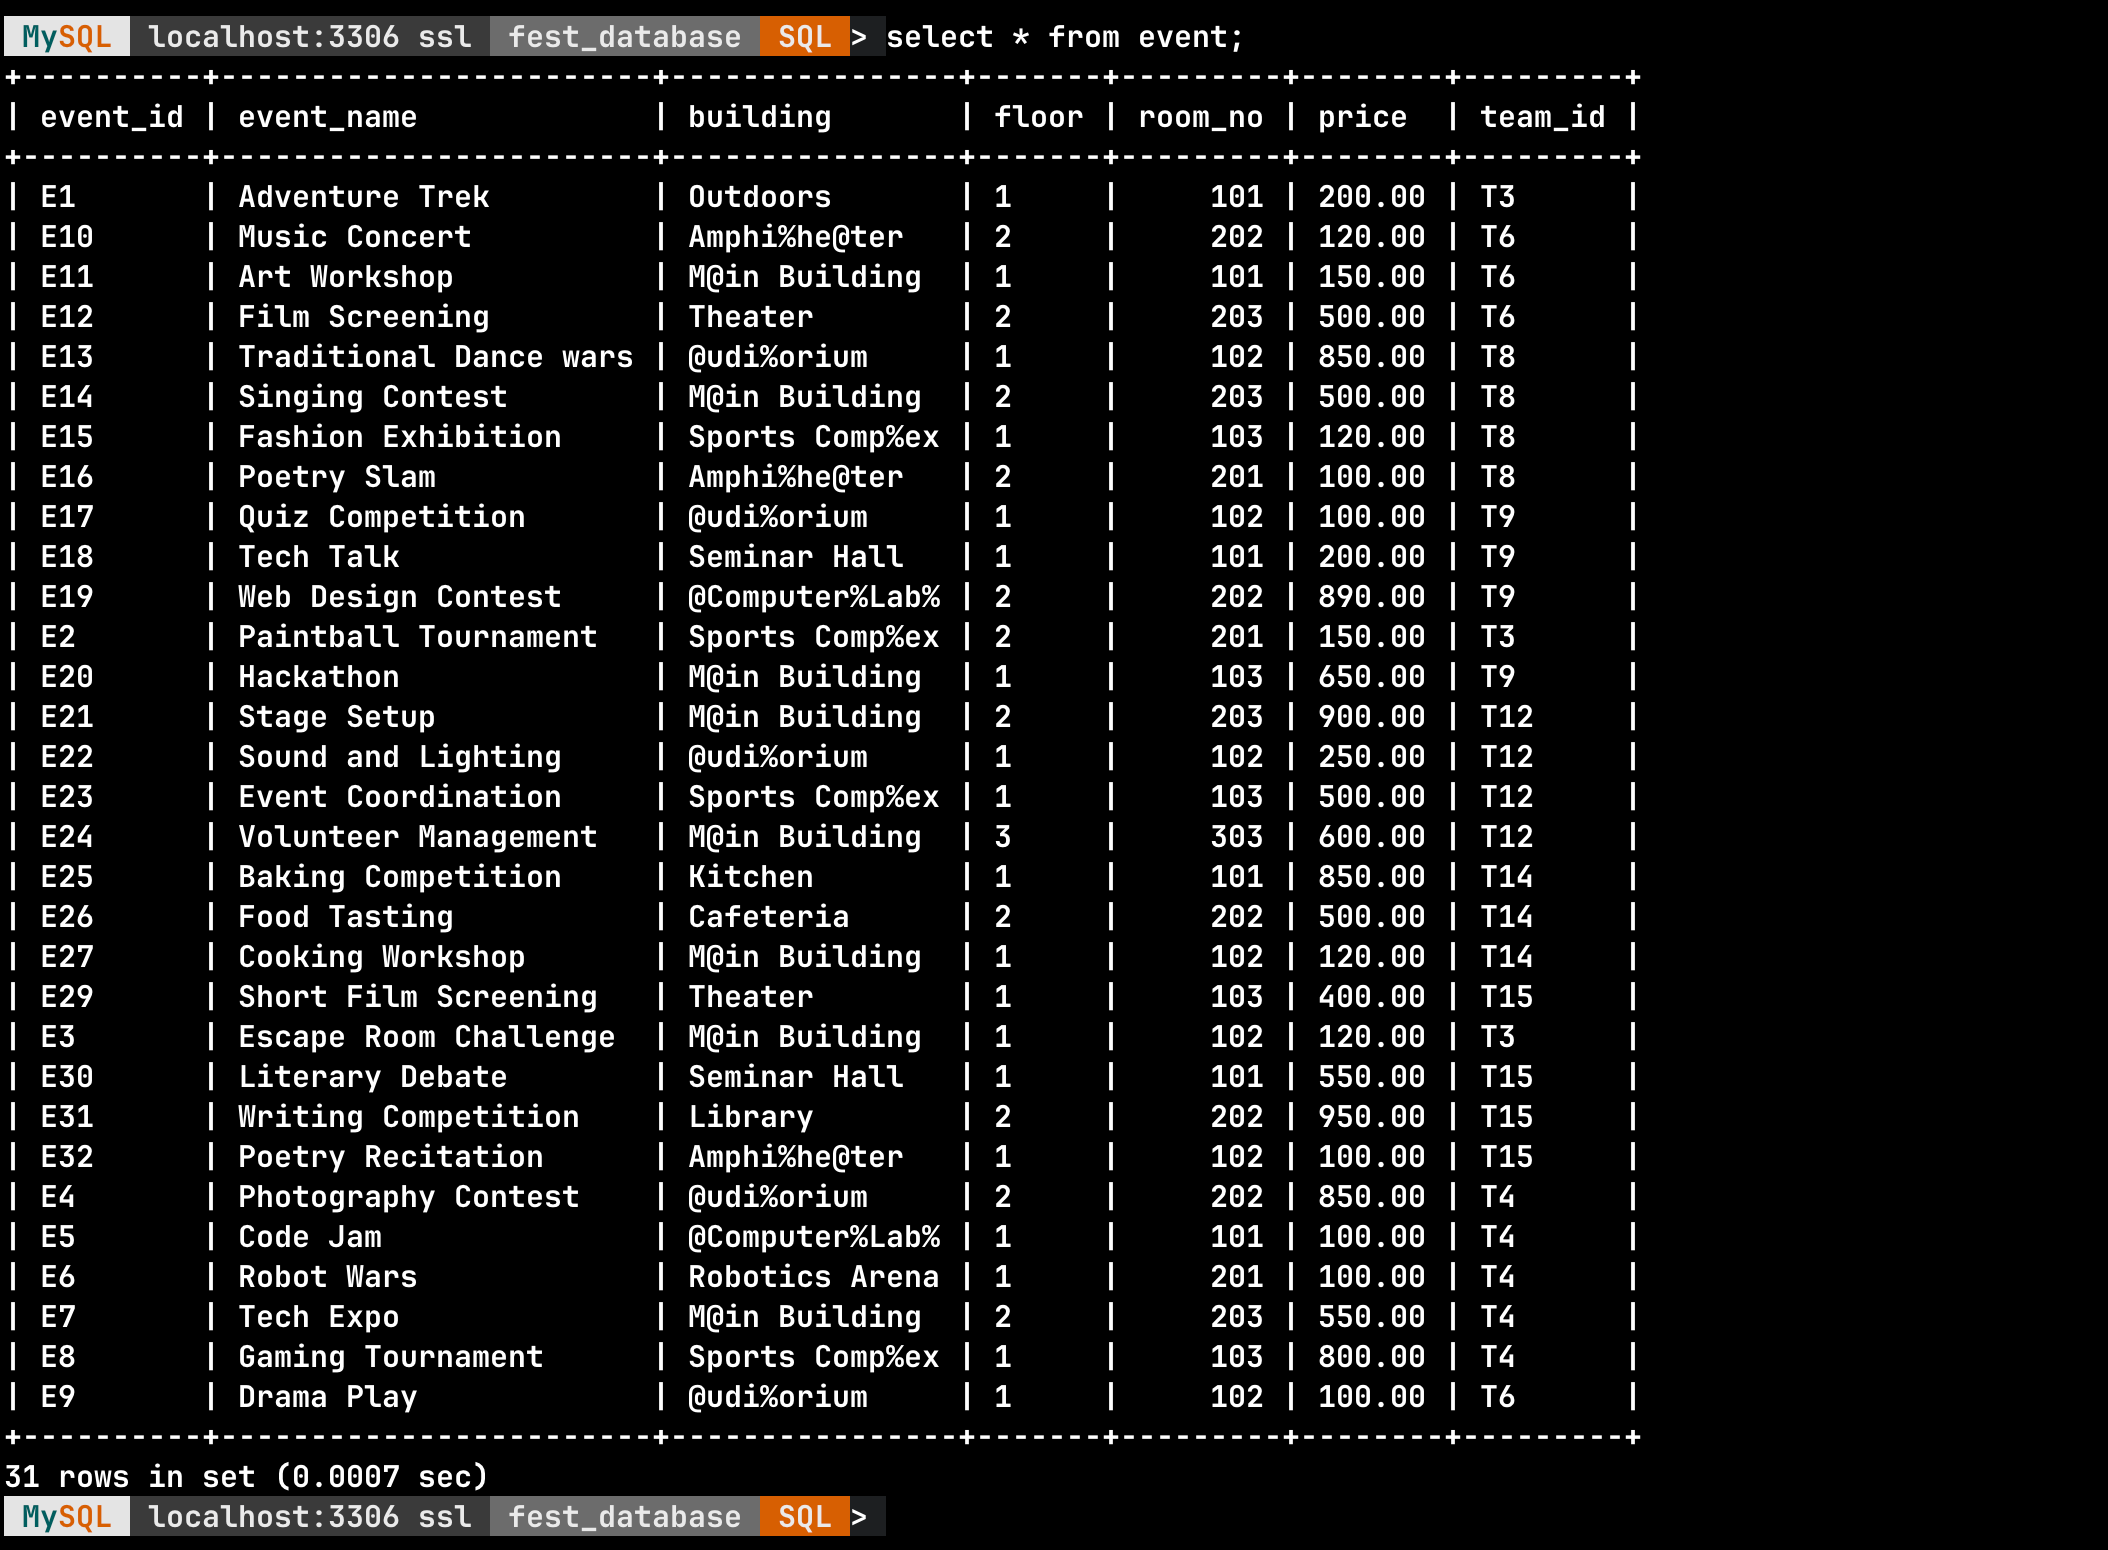
\includegraphics[width=0.9\linewidth]{./images/task1/1a.png}
\end{figure}

\begin{figure}[H]
    \centering 
    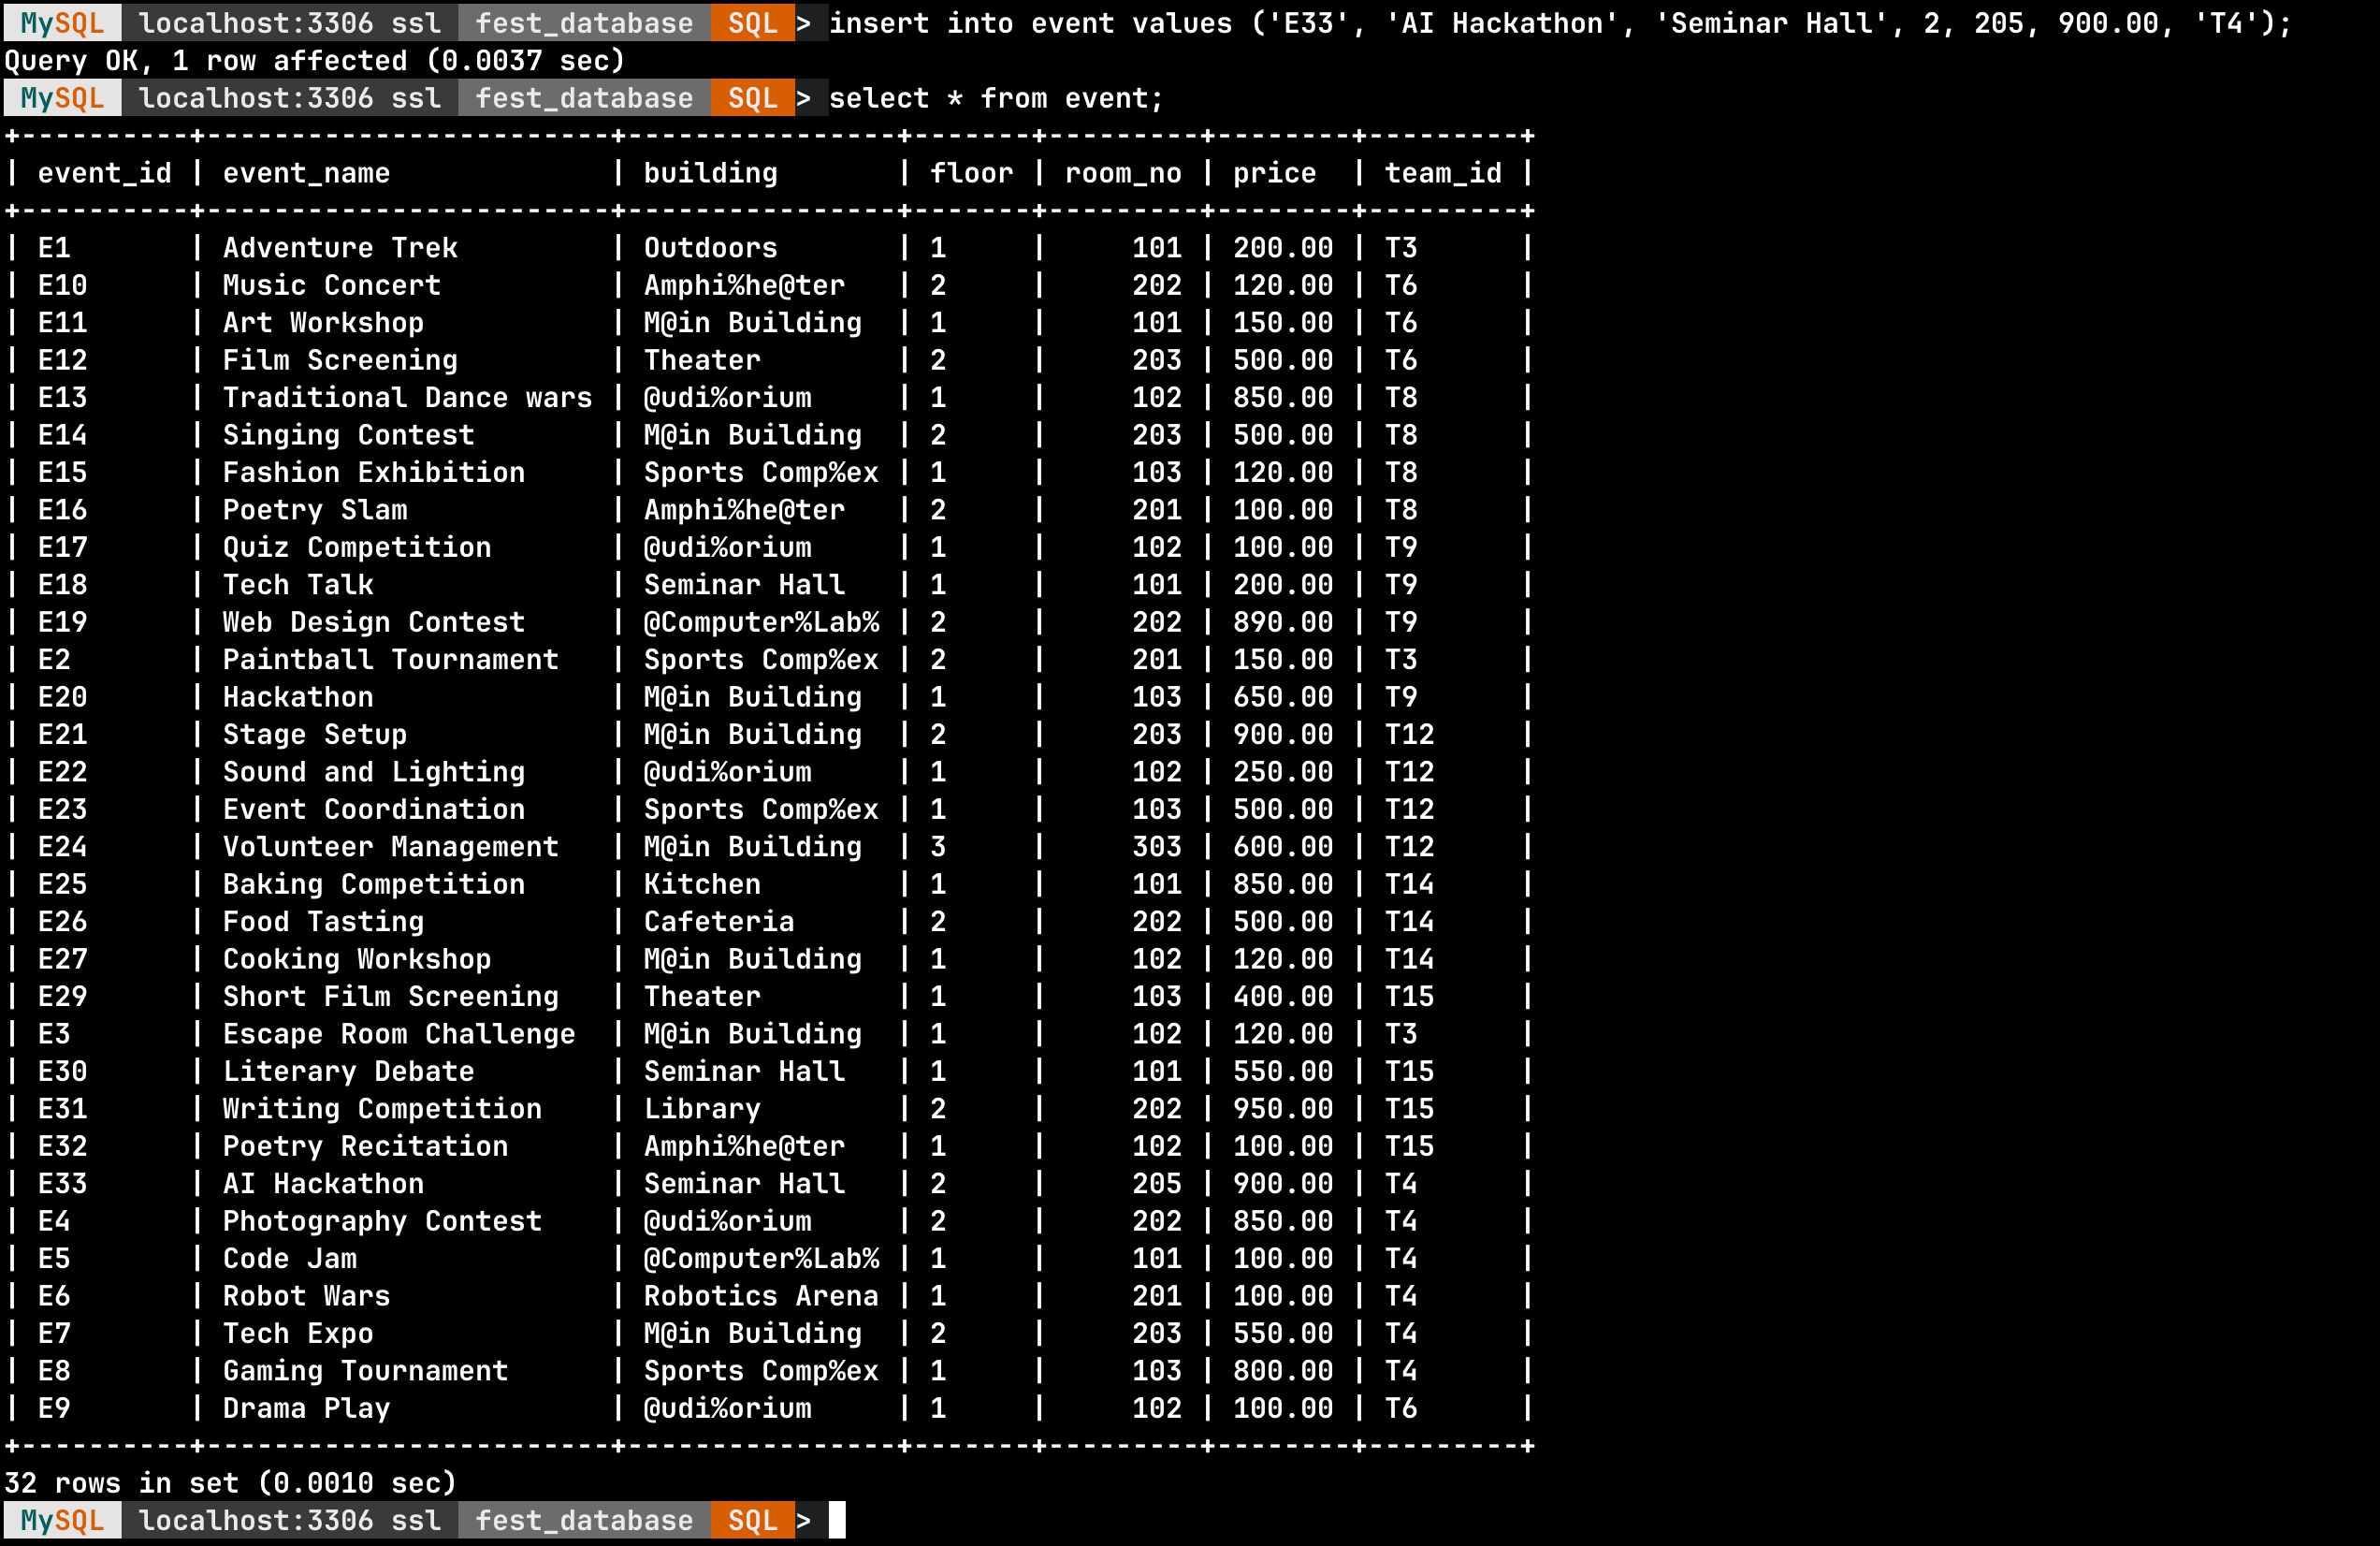
\includegraphics[width=0.9\linewidth]{./images/task1/1b.png}
\end{figure}

2. Update the quantity of ``Mushroom Risotto'' in stall ``S1'' to 25.

\begin{figure}[H]
    \centering 
    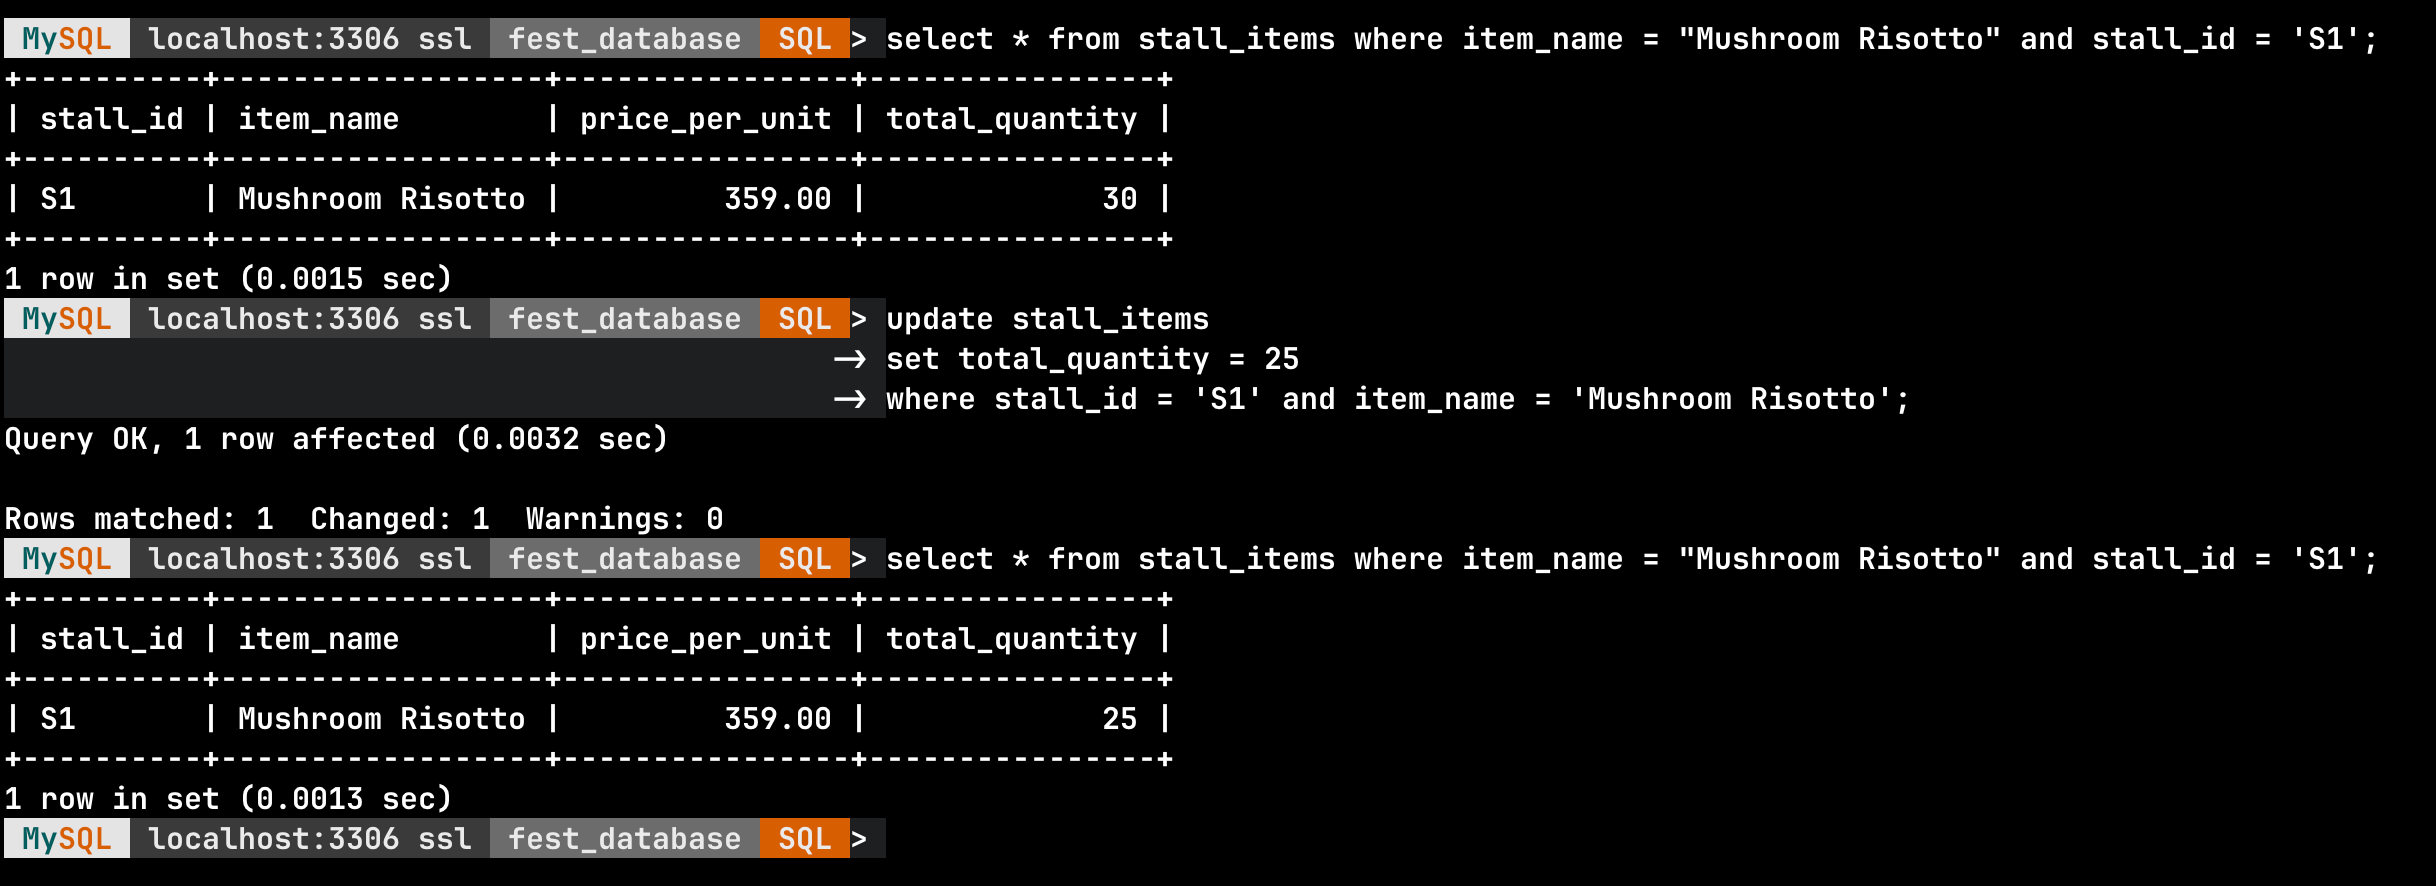
\includegraphics[width=0.9\linewidth]{./images/task1/2.png}
\end{figure}

3. Delete all registrations where the event ID is \texttt{E1} and SRN starts with \texttt{P100}.

\begin{figure}[H]
    \centering 
    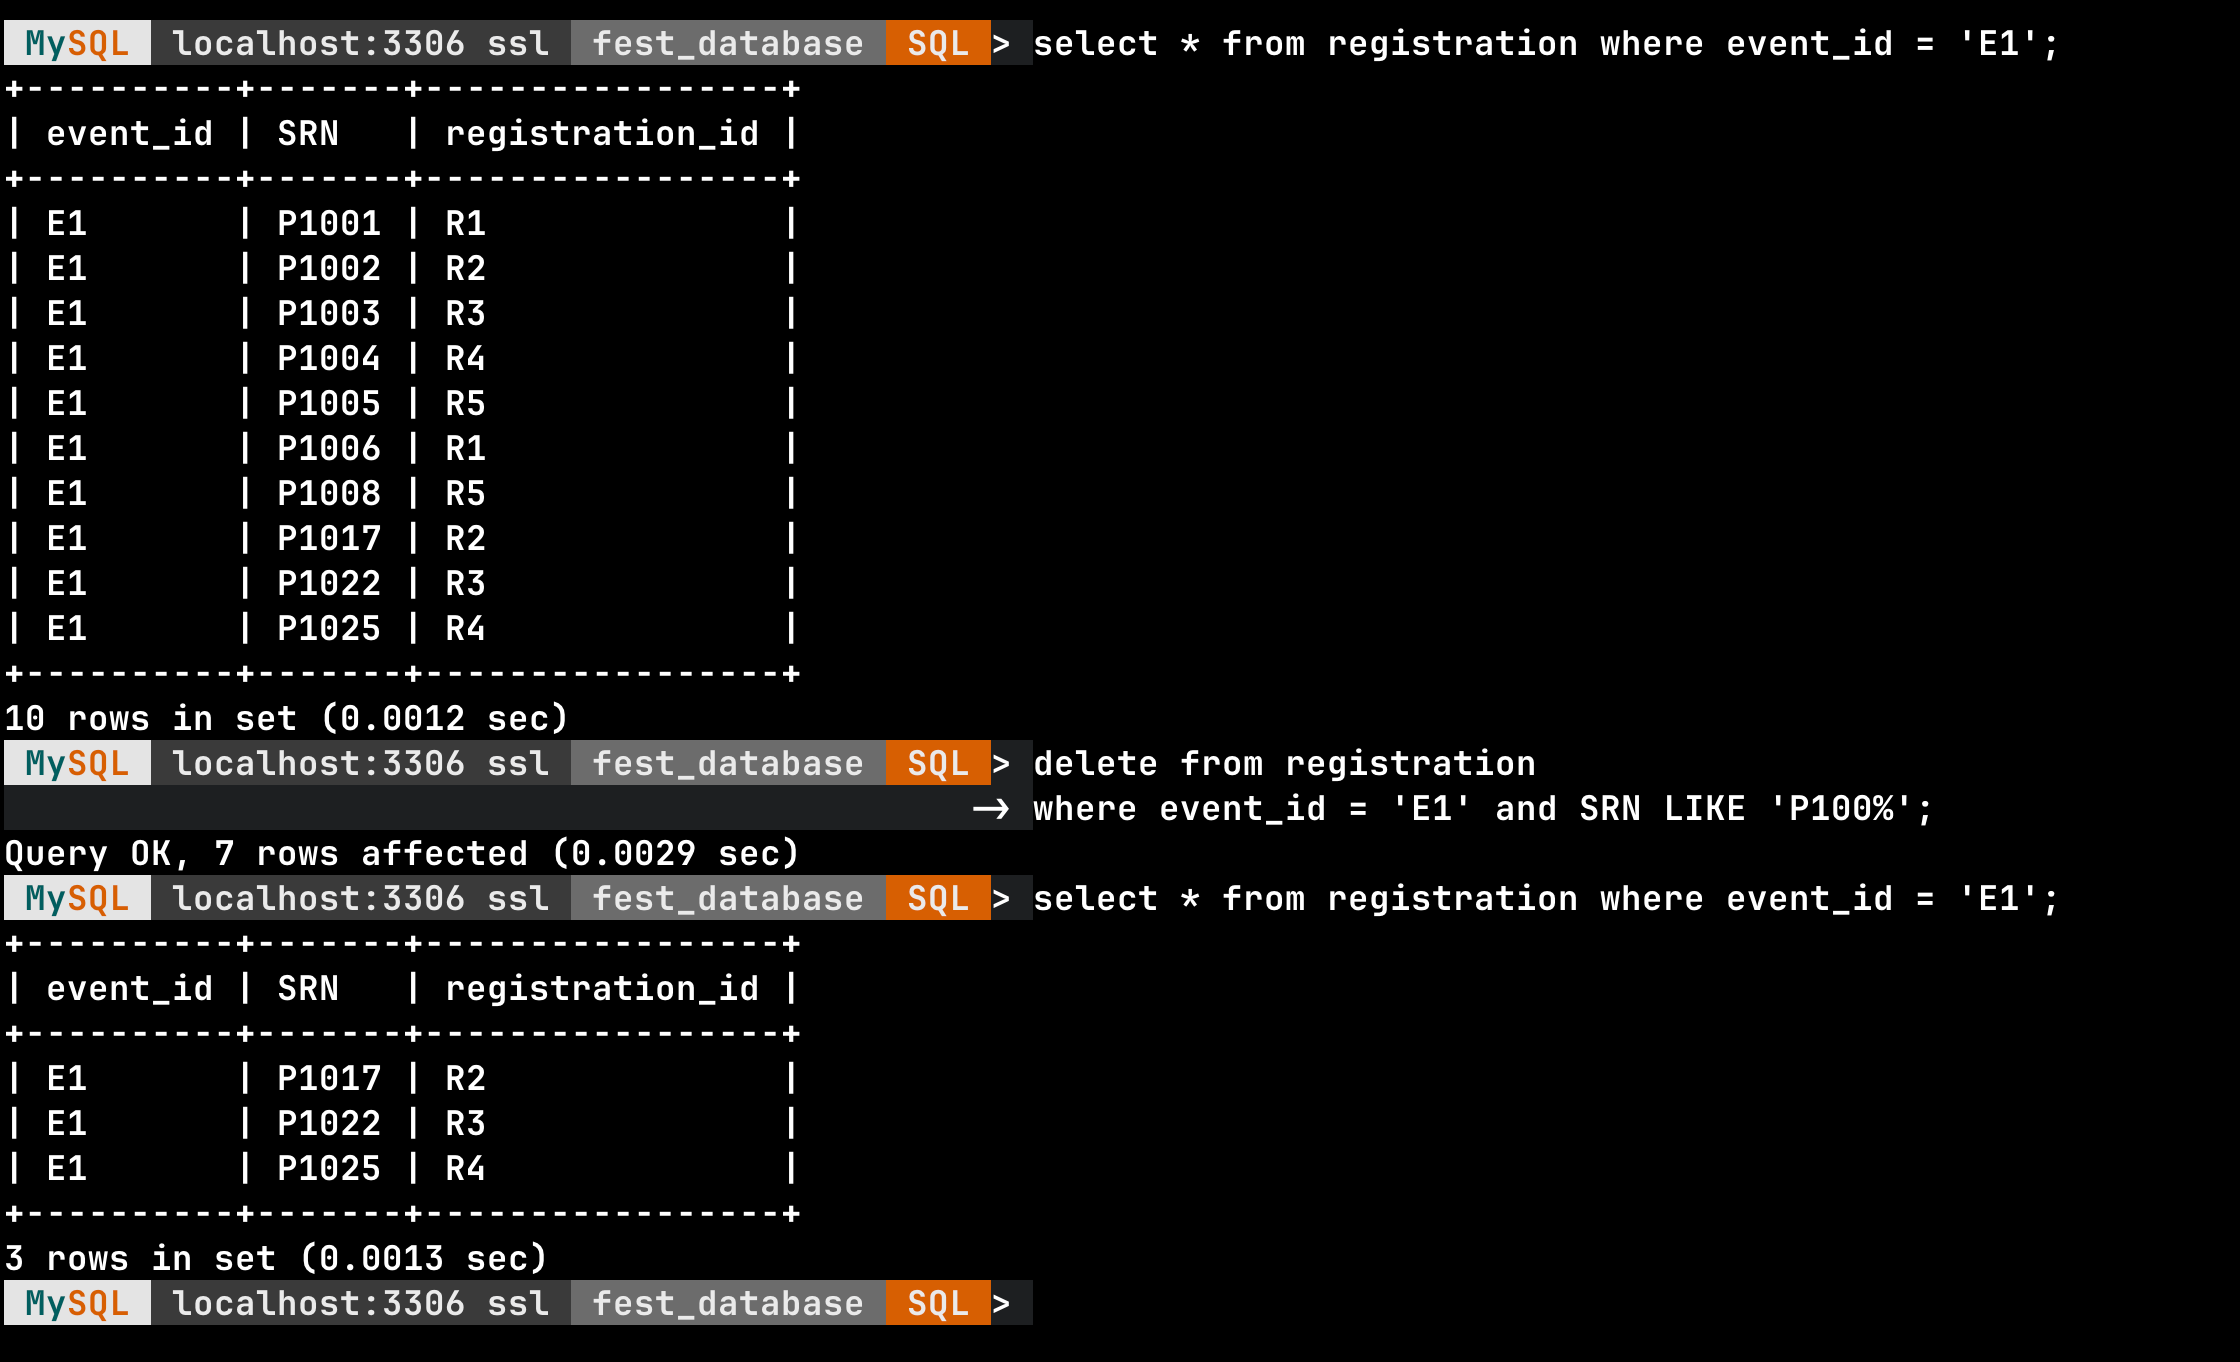
\includegraphics[width=0.9\linewidth]{./images/task1/3.png}
\end{figure}

4. Insert a new purchase: \texttt{P1017} buys 3 \texttt{Fish Tacos} from stall \texttt{S6} at \texttt{2025\-07\-10 14:00:00}.

\begin{figure}[H]
    \centering 
    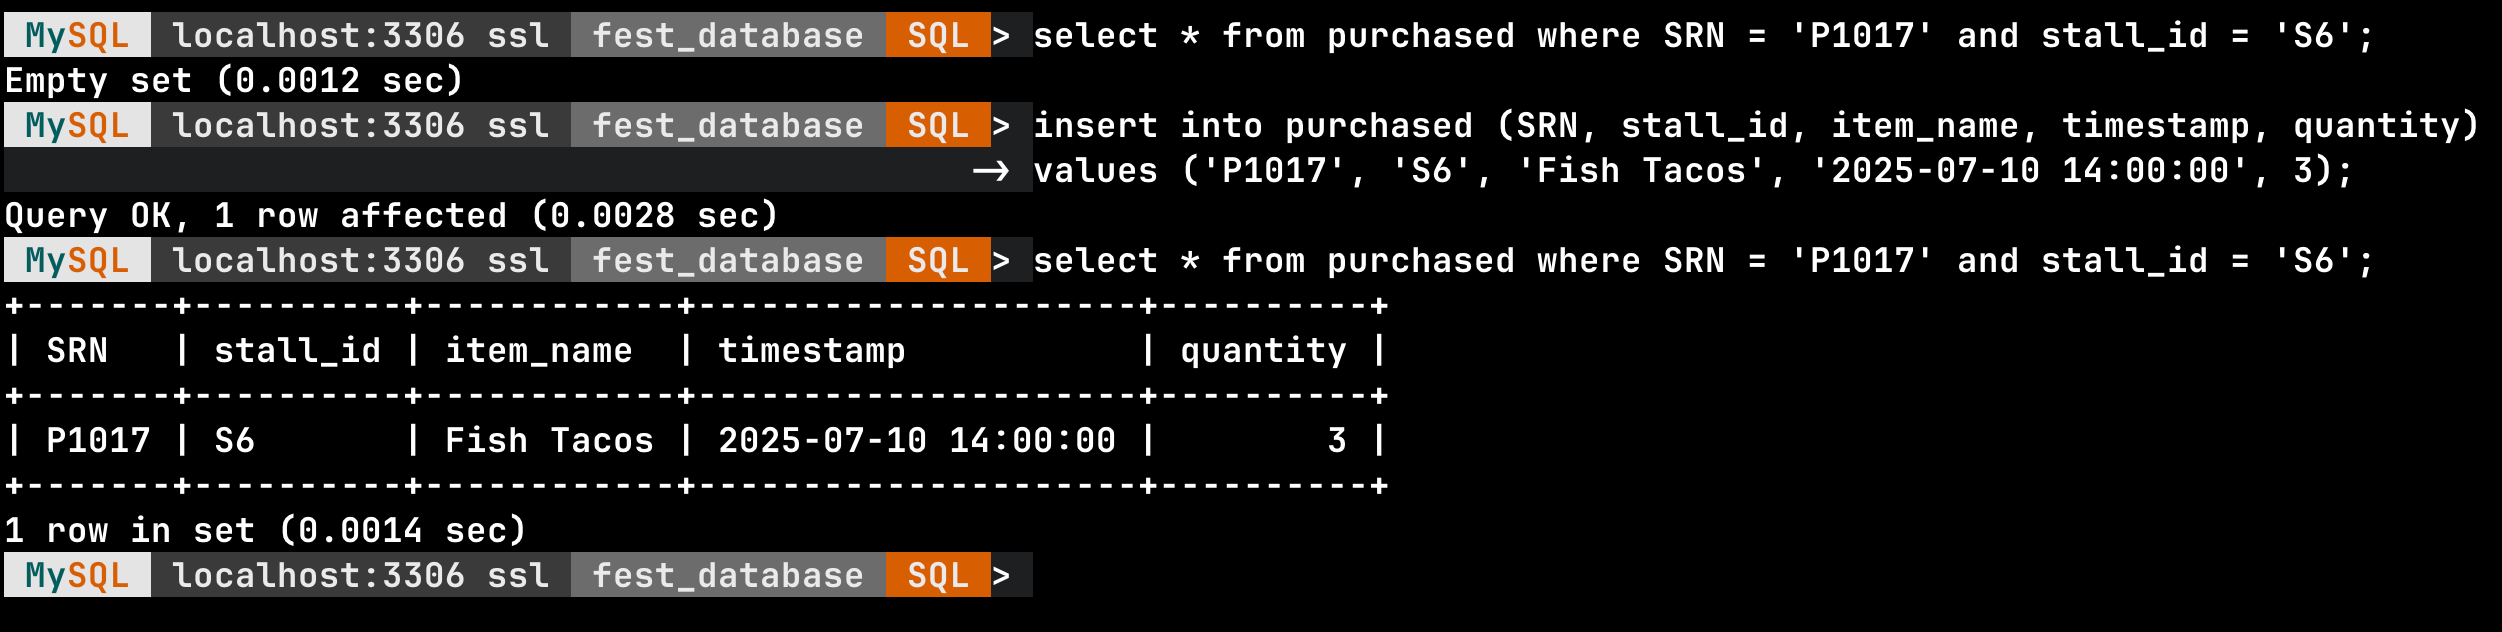
\includegraphics[width=0.9\linewidth]{./images/task1/4.png}
\end{figure}

\pagebreak

5. Retrieve participants's SRN who are registered only for event \texttt{E2} or \texttt{E5}, but not both (using SET operations).

\begin{figure}[H]
    \centering 
    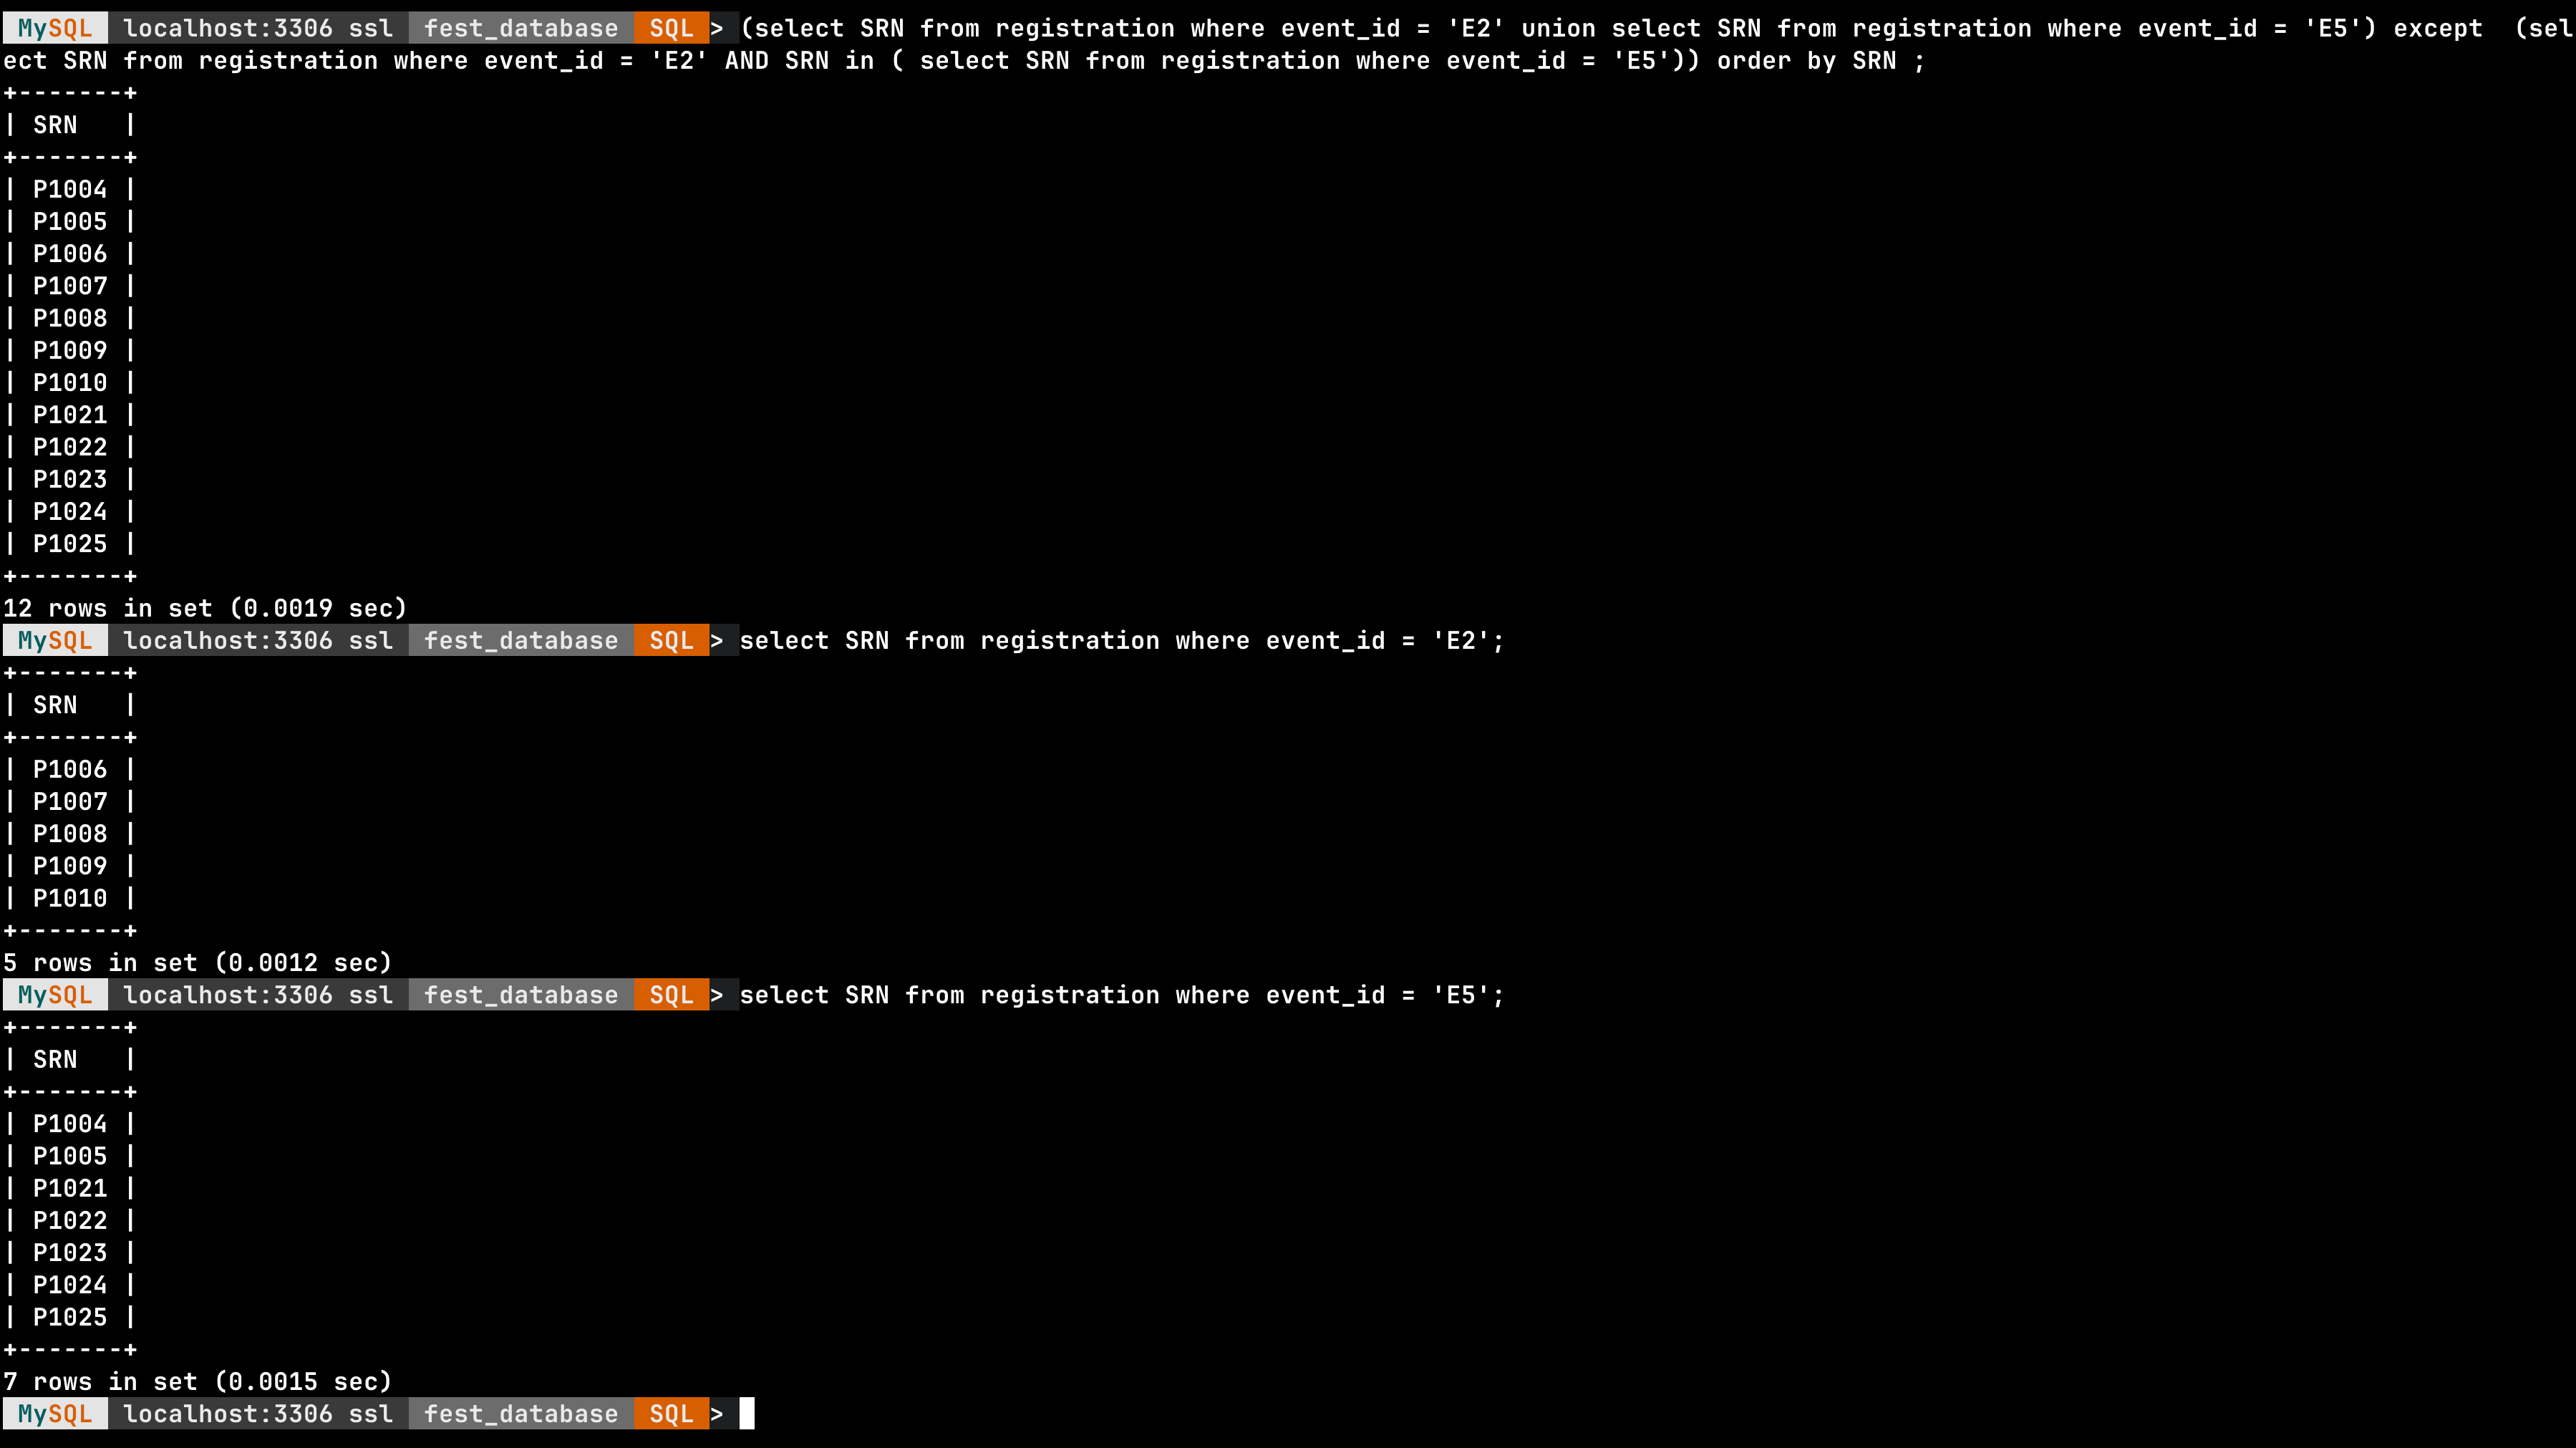
\includegraphics[width=0.9\linewidth]{./images/task2/5.png}
\end{figure}

6. Display all participants and the names of all their visitors (if any) with a count of visitors.

\begin{figure}[H]
    \centering 
    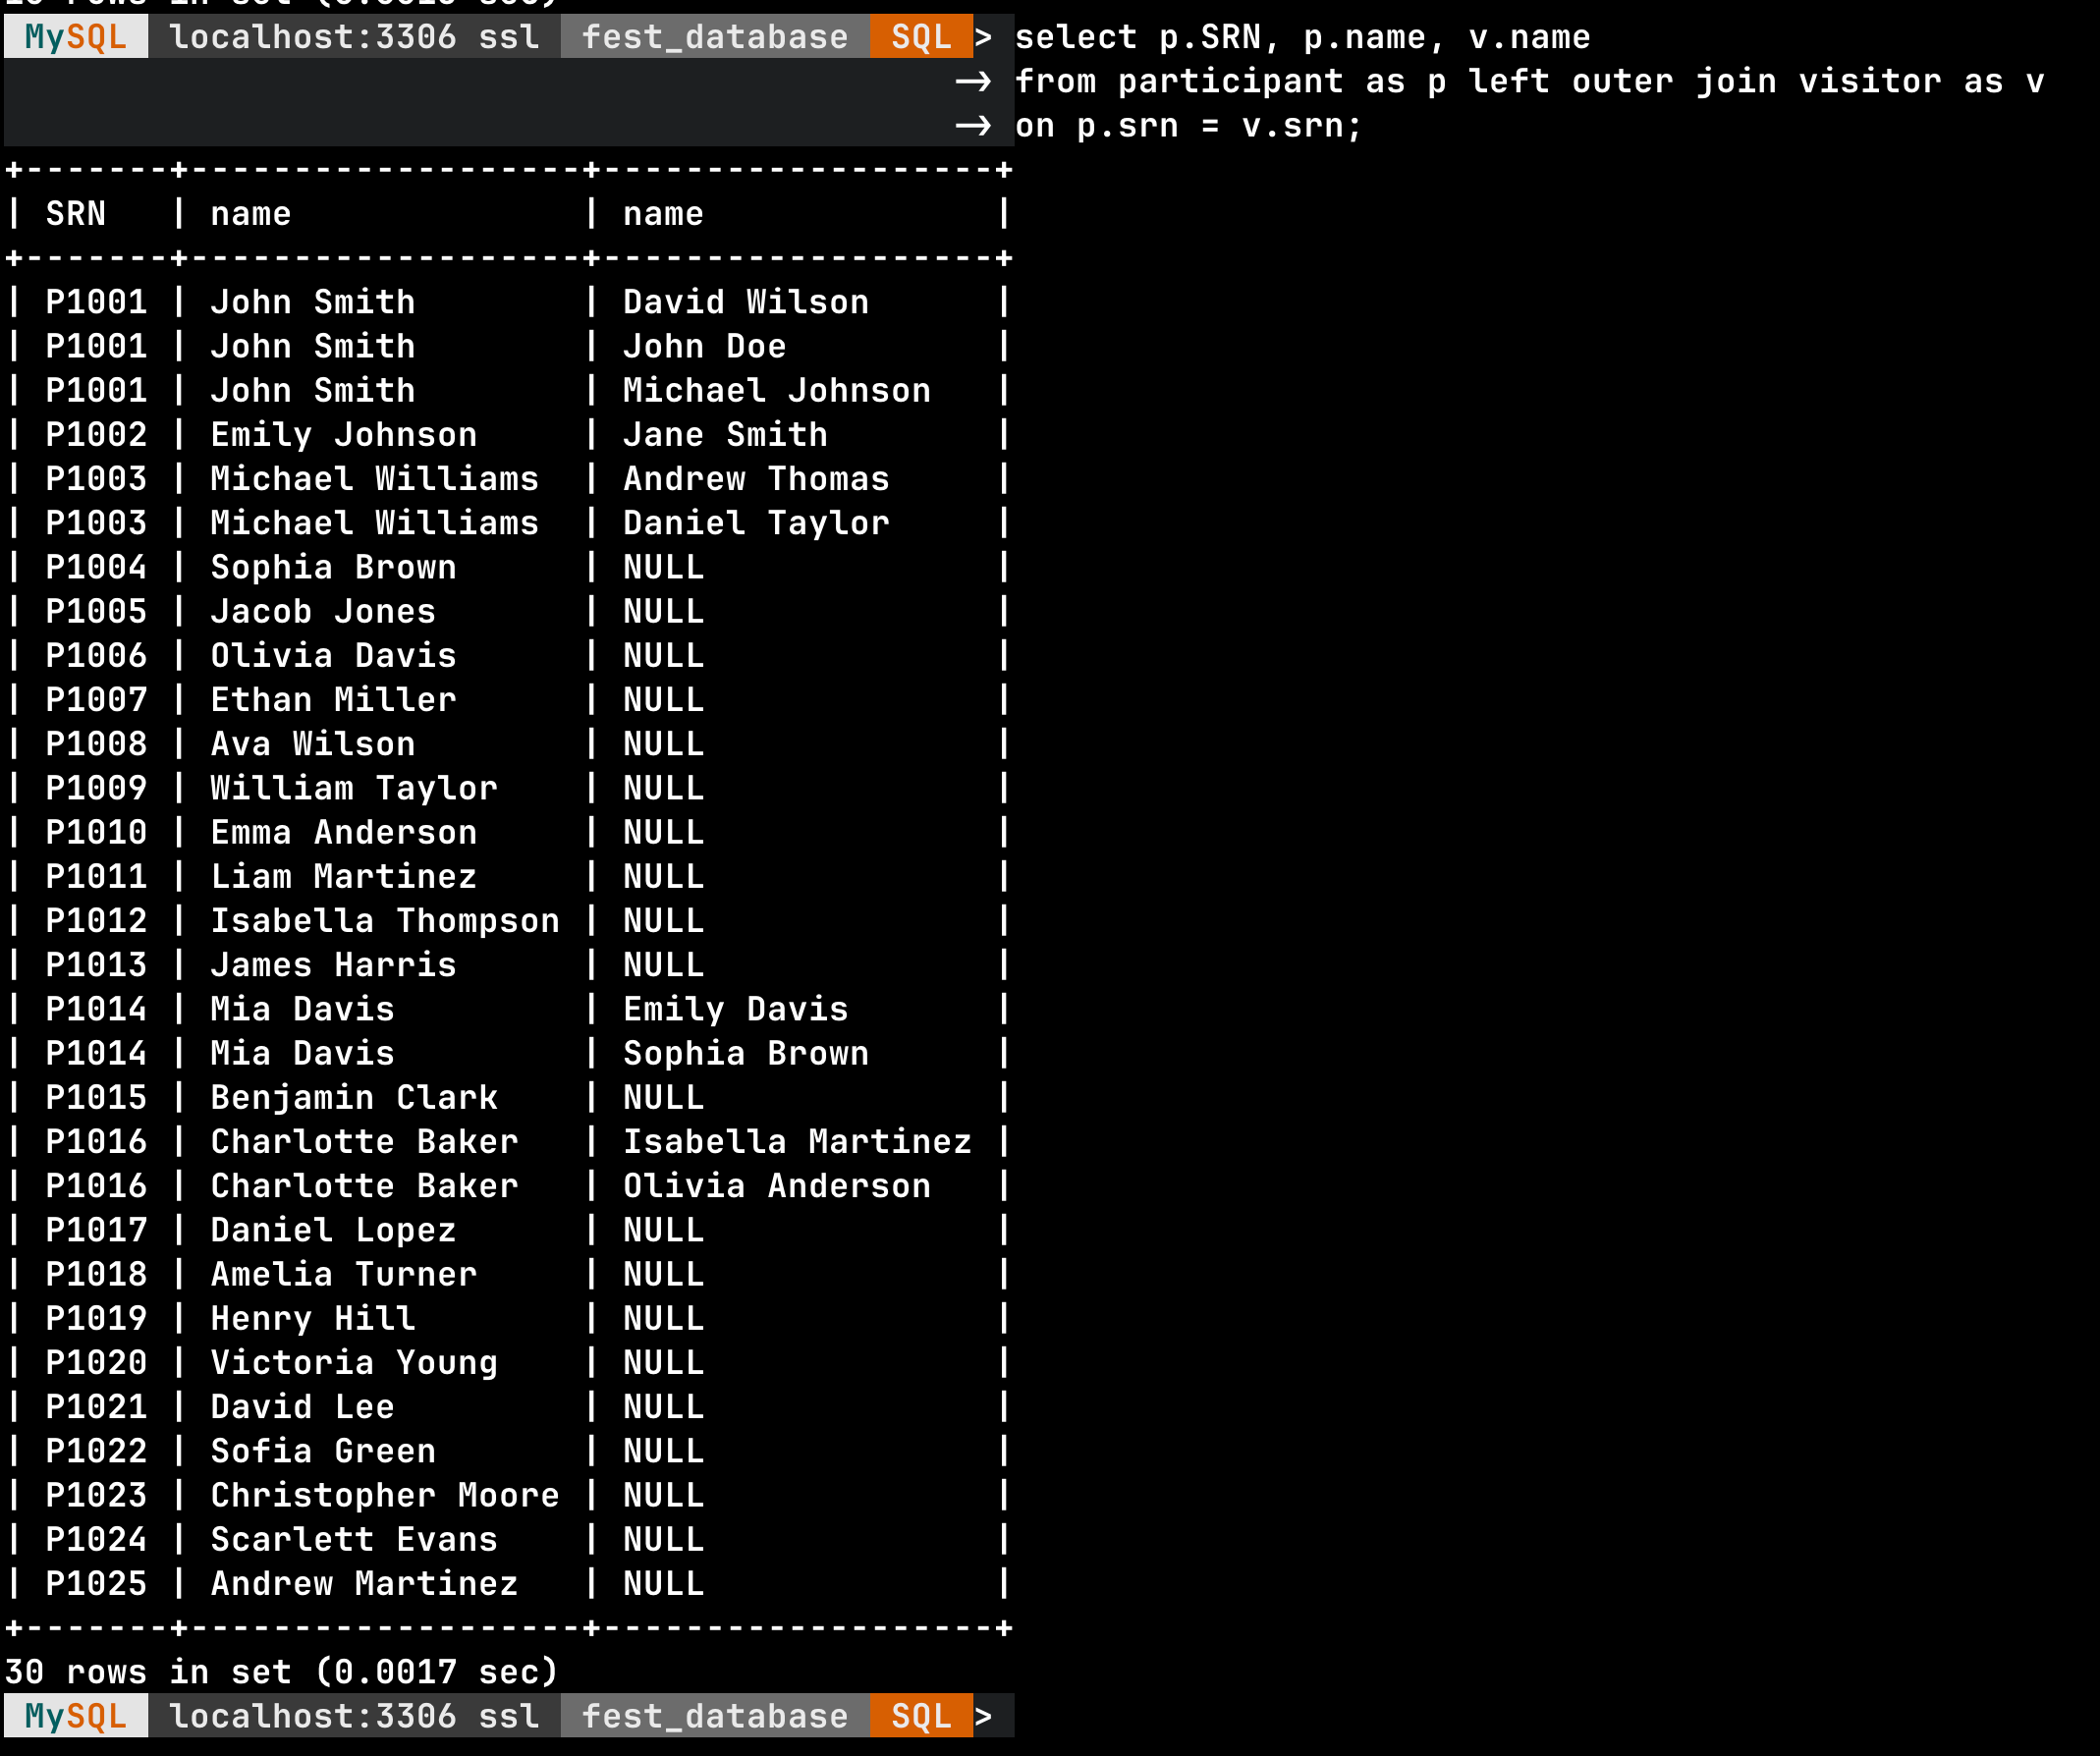
\includegraphics[width=0.9\linewidth]{./images/task2/6.png}
\end{figure}

7. List events that have equal number of male and female participants.

\begin{figure}[H]
    \centering 
    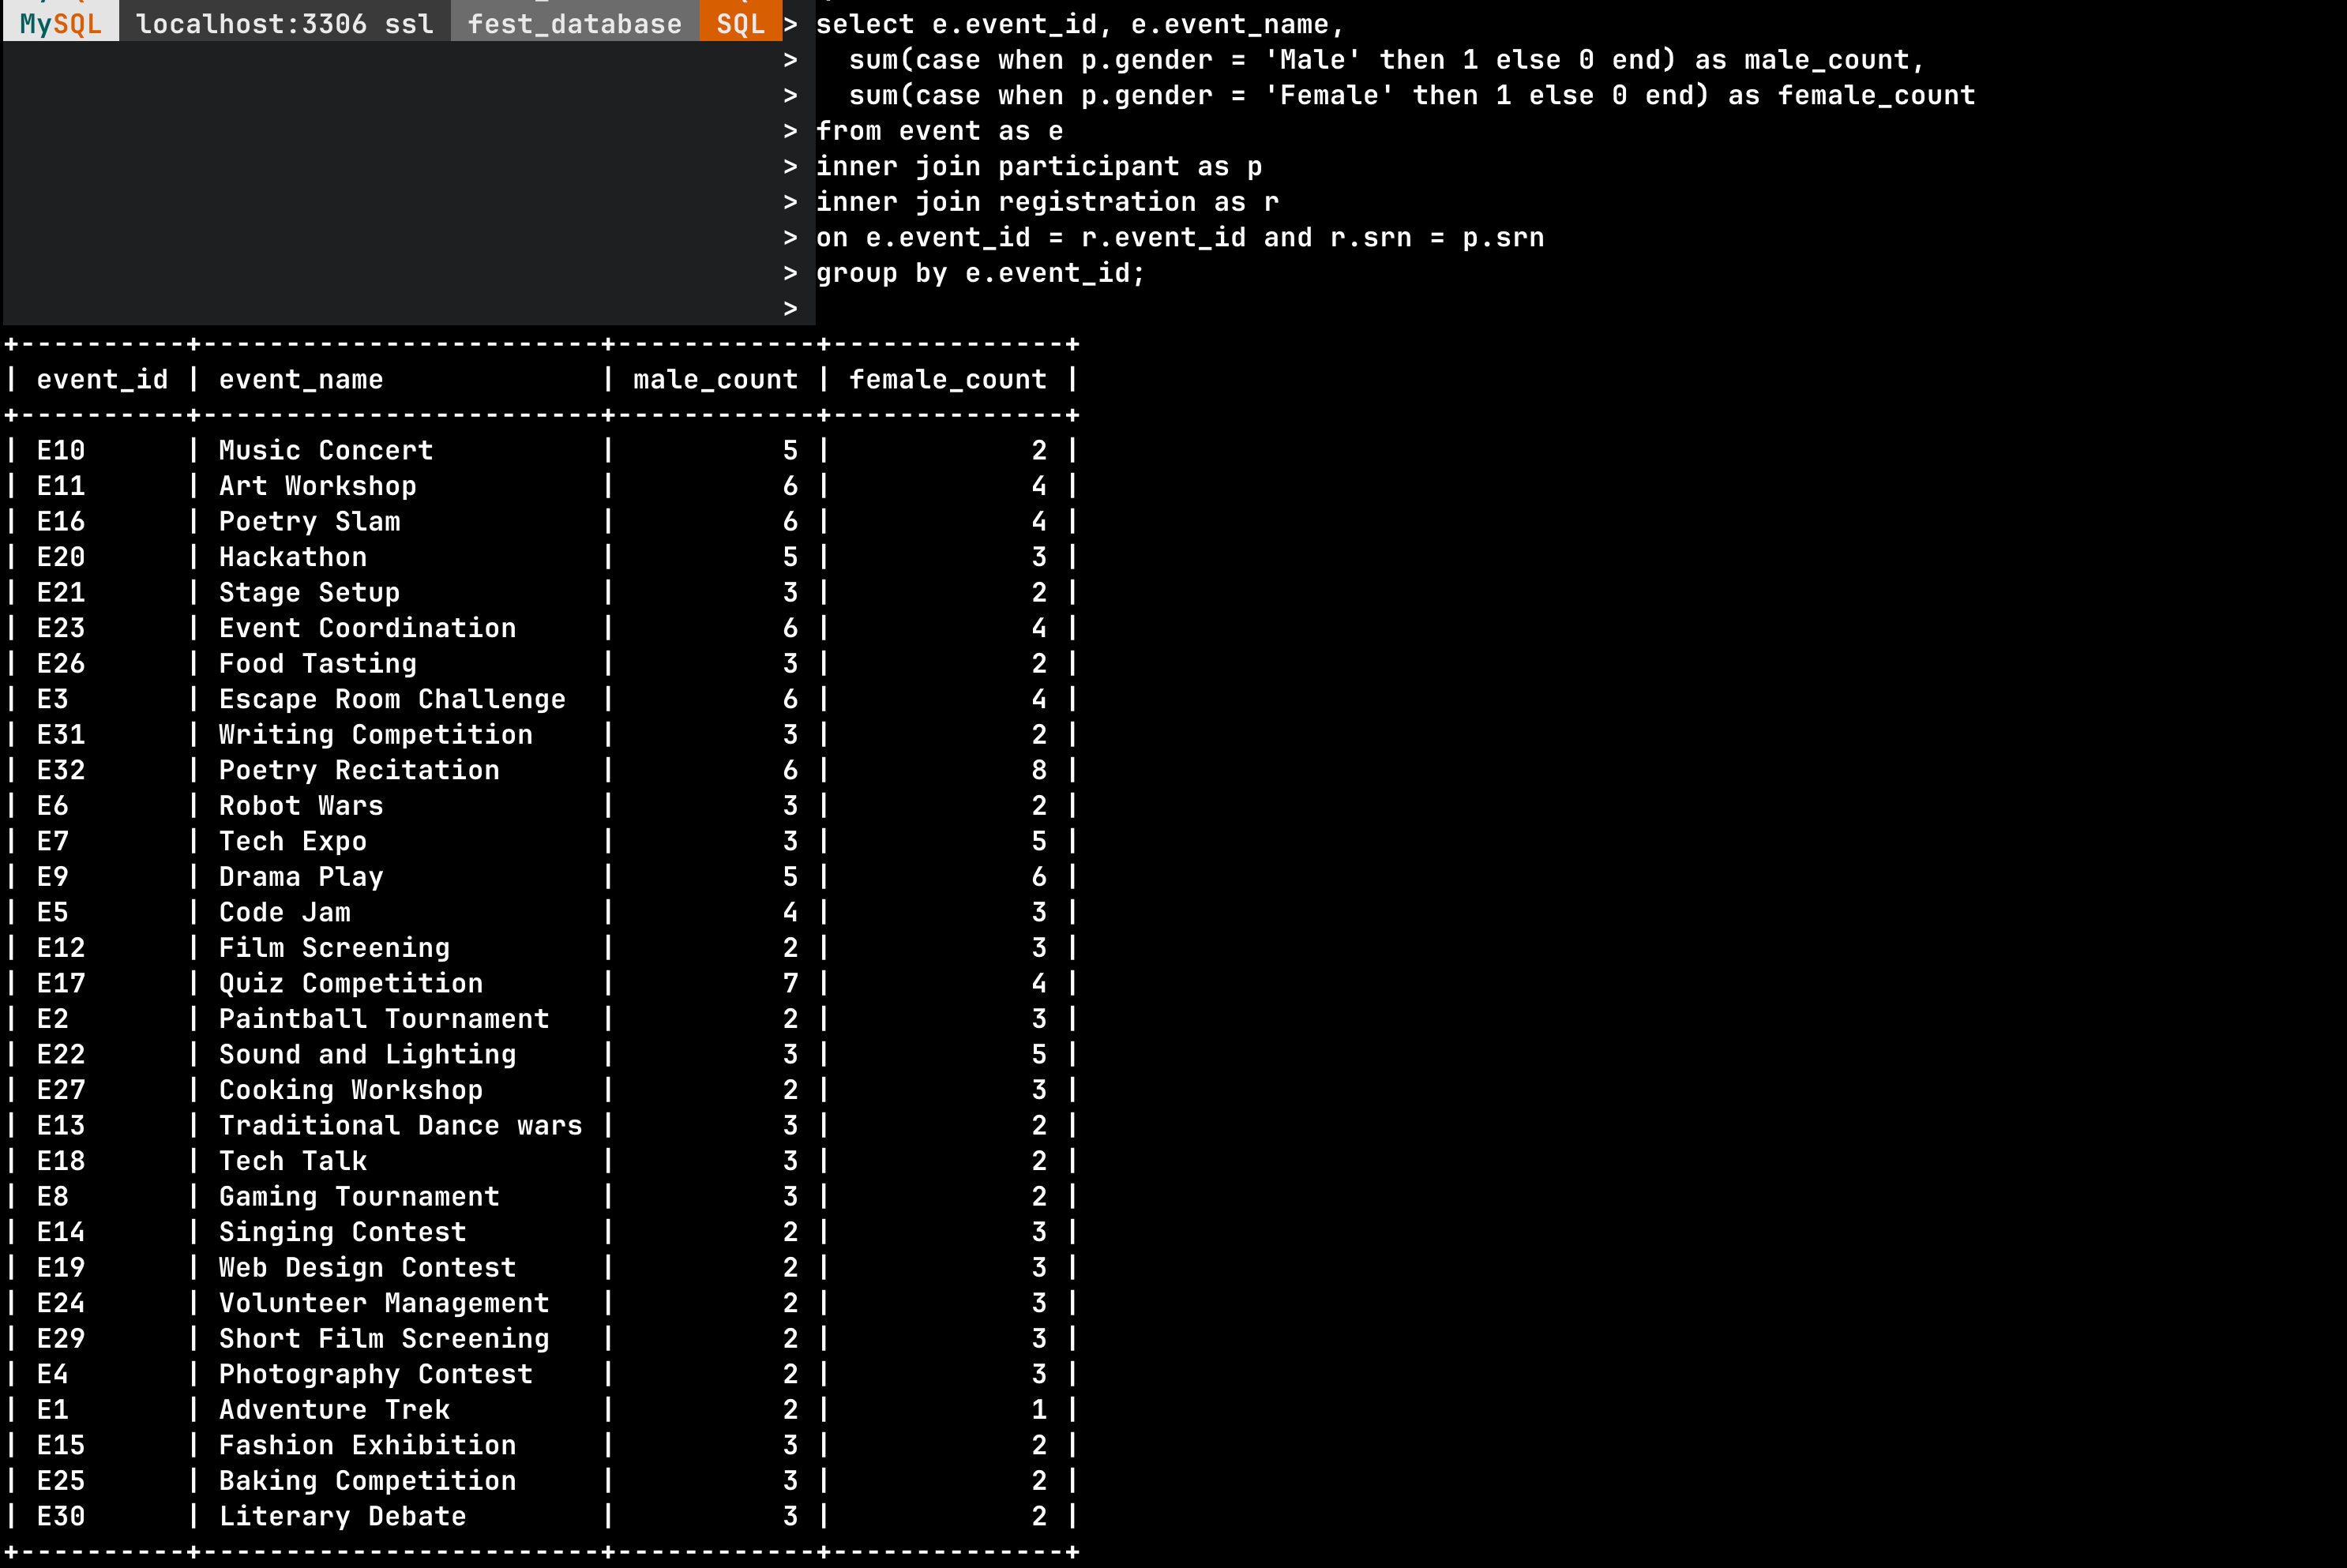
\includegraphics[width=0.9\linewidth]{./images/task2/7a.png}
\end{figure}

\begin{figure}[H]
    \centering 
    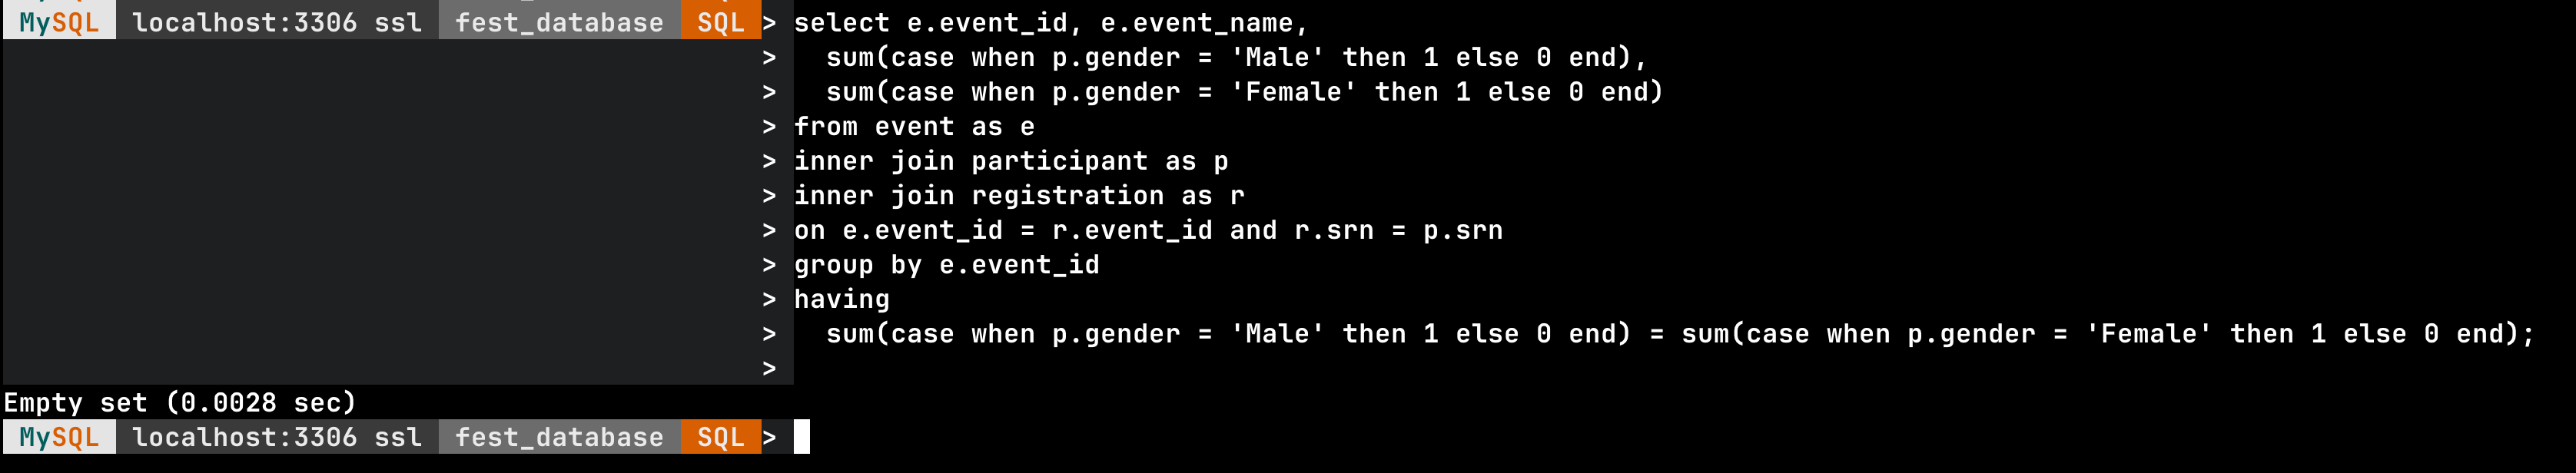
\includegraphics[width=0.9\linewidth]{./images/task2/7b.png}
\end{figure}

8. Display each event's name and a binary indicator of whether it occurred after the Golden Jubilee ($\mathit{year} < 2047$).

\begin{figure}[H]
    \centering 
    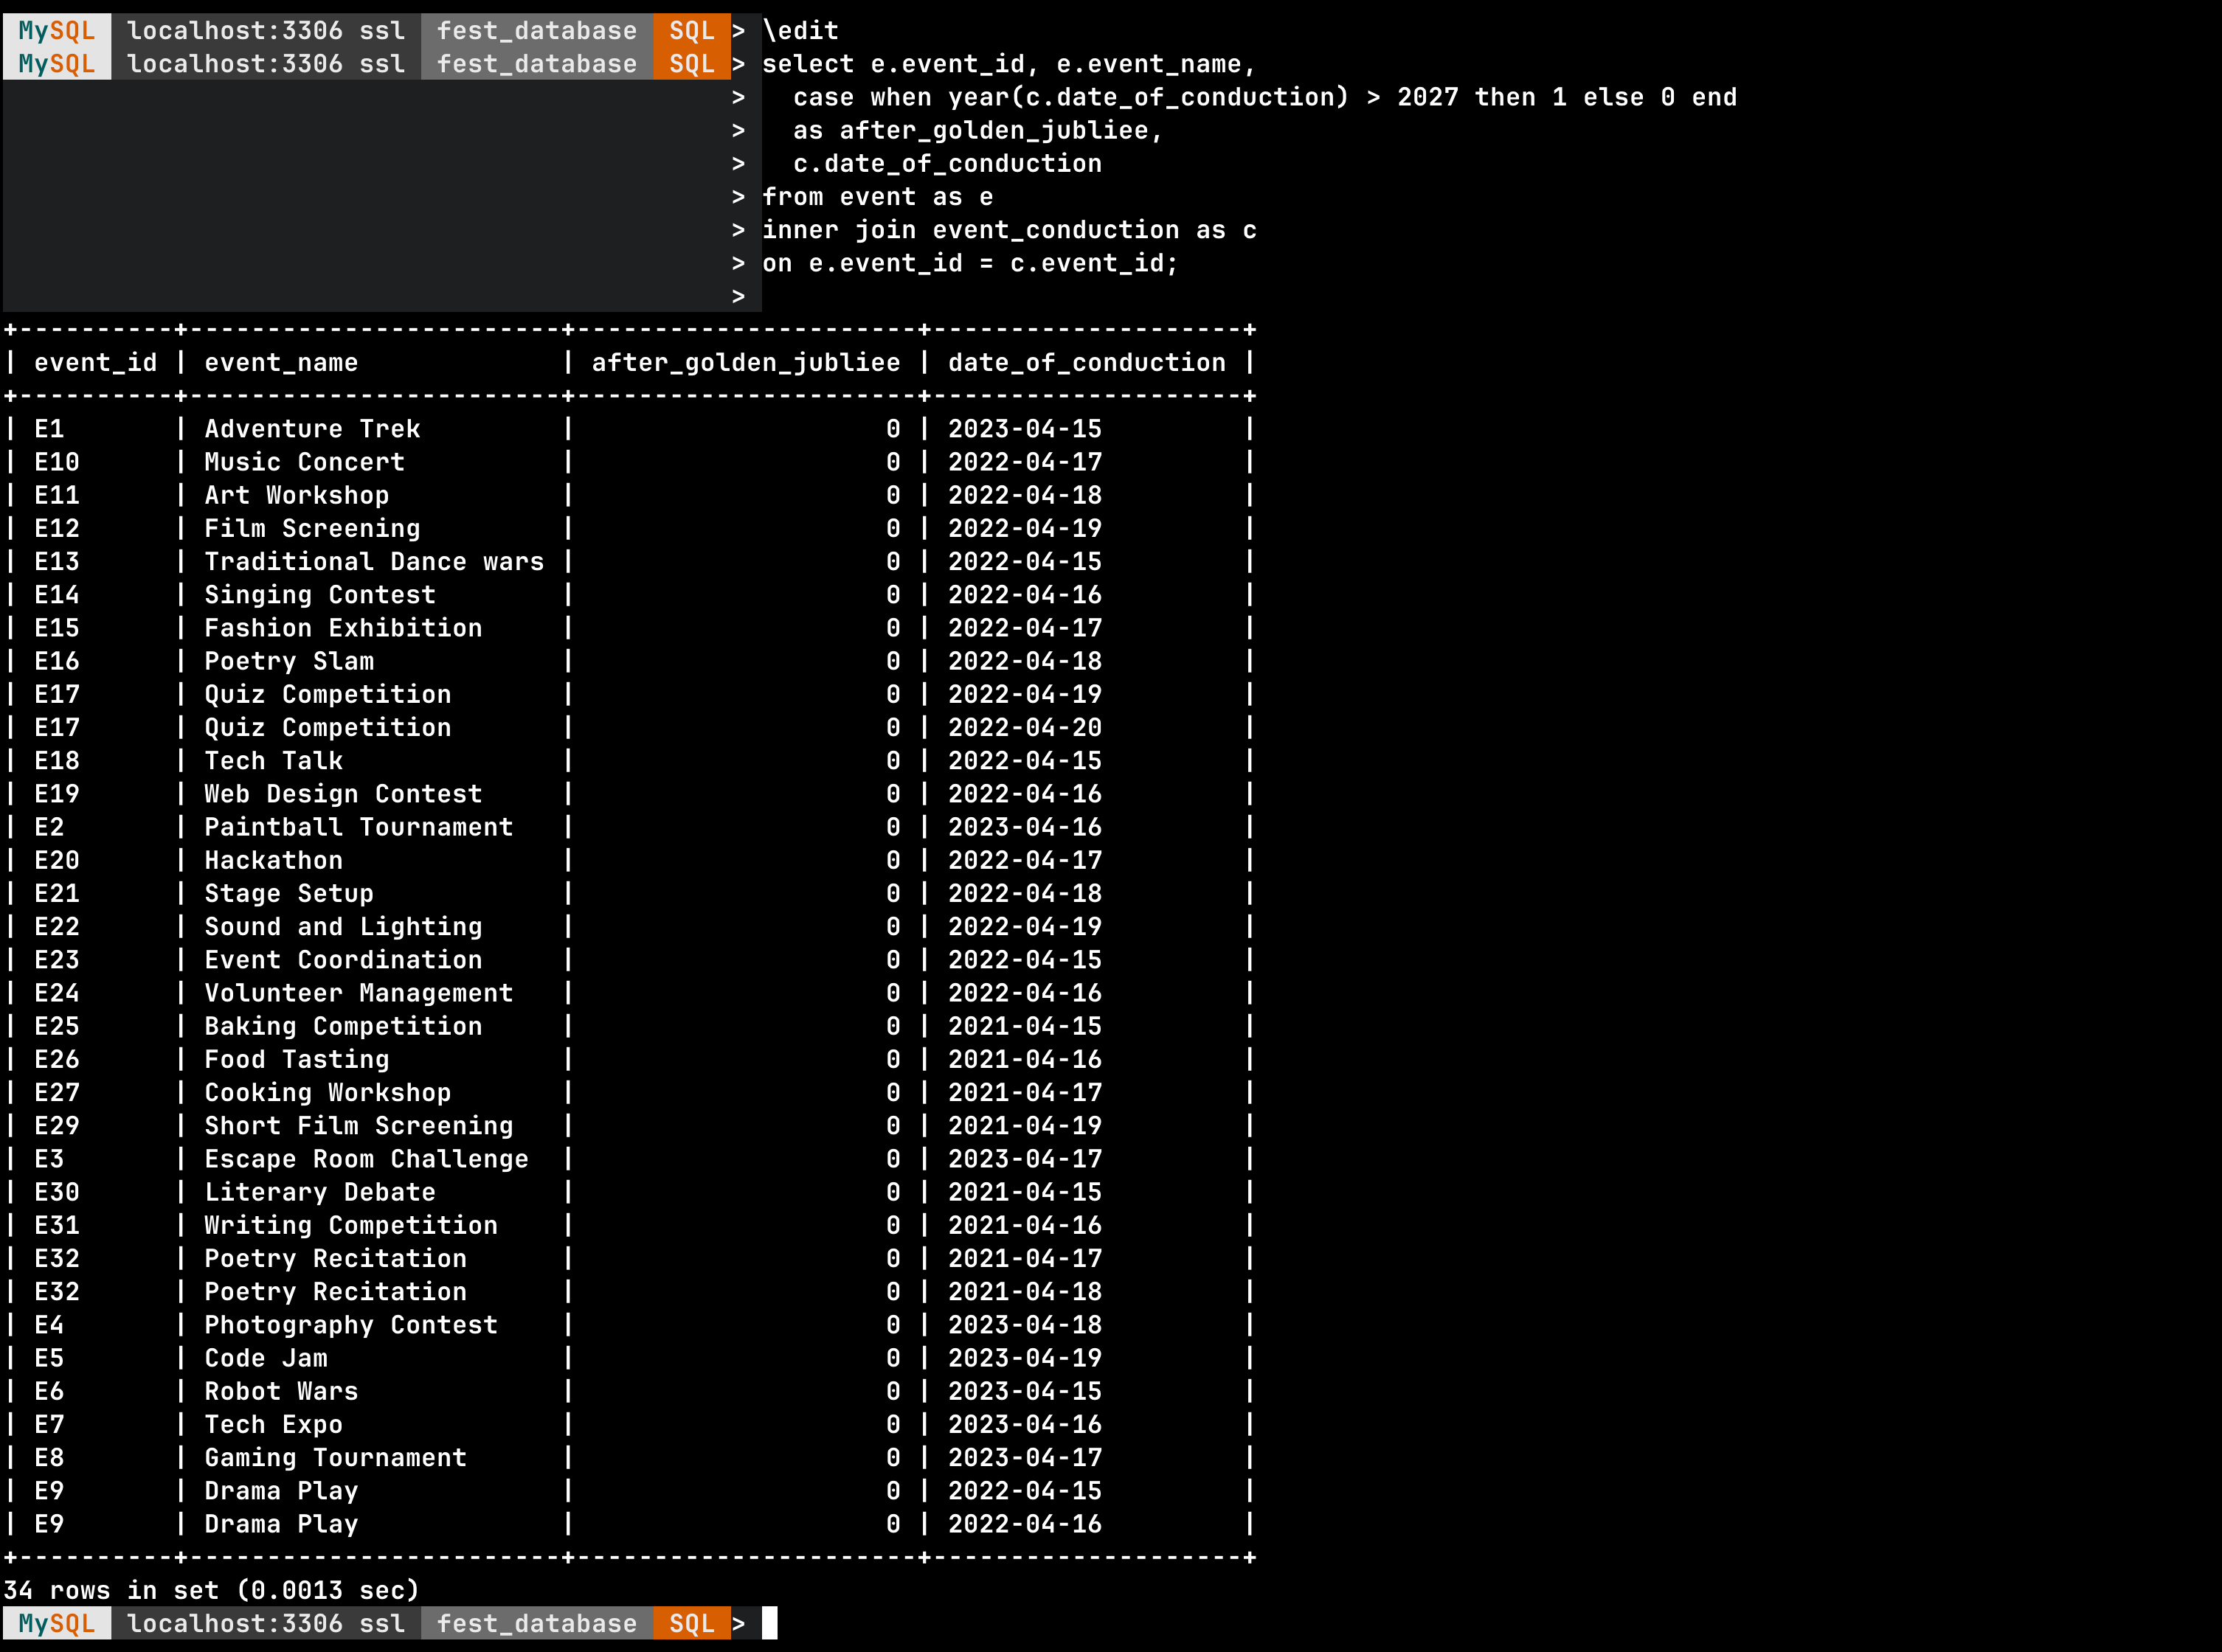
\includegraphics[width=0.9\linewidth]{./images/task2/8.png}
\end{figure}

\pagebreak

\section{Task 3}

\begin{itemize}
\item Which SQL command is used to insert new records into a table \\
The insert into command is used to insert new records into a table.
    \begin{minted}{SQL}
INSERT INTO table_name
[(column1, column2, column3, ...)] 
VALUES (value1, value2, value3, ...);
    \end{minted}
\item What is the difference between DELETE and TRUNCATE in SQL\@?
\begin{itemize}
    \item \texttt{DELETE}: Removes specific rows from a table based on a condition. It can be rolled back if within a transaction.
    \item \texttt{TRUNCATE}: Removes all rows from a table, resetting it to empty. It is faster than DELETE but cannot be rolled back.
\end{itemize}

\item Which DML command is used to modify existing values in a table \\
The \texttt{UPDATE} command is used to modify existing values in a table.

\item Can a single INSERT statement add multiple rows at once \\
Yes, a single \texttt{INSERT} statement can add multiple rows at once by specifying multiple sets of values.

\item Which DML command is used to fetch records from one or more tables \\
The \texttt{SELECT} command is used to fetch records from one or more tables.

\item What is the purpose of using a JOIN in SQL\@? \\
The purpose of using a \texttt{JOIN} in SQL is to combine rows from two or more tables based on a related column between them, allowing for the retrieval of related data in a single query.

\item Which JOIN returns only the rows that have matching values in both tables \\ 
The \texttt{INNER JOIN} returns only the rows that have matching values in both tables.

\item What does a LEFT JOIN return when there is no matching row in the right table \\
A \texttt{LEFT JOIN} returns all rows from the left table and the matched rows from the right table. If there is no match, NULL values are returned for columns from the right table.

\item Can MySQL directly perform a FULL OUTER JOIN\@? If not, how can it be achieved

MySQL does not directly support \texttt{FULL OUTER JOIN}. However, it can be achieved by combining a \texttt{LEFT JOIN} and a \texttt{RIGHT JOIN} using a \texttt{UNION} operation.

\item What is the difference between INNER JOIN and CROSS JOIN\@?
\begin{itemize}
    \item \texttt{INNER JOIN}: Returns only the rows that have matching values in both tables based on a specified condition.
    \item \texttt{CROSS JOIN}: Returns the Cartesian product of both tables, combining each row from the first table with every row from the second table, resulting in all possible combinations. 
\end{itemize}
\end{itemize}

\end{document}